%% ===================================================================
%% ISCAS 2027 submission -- 4 pages + 1 page references.
%% Rebuilt 2026-09-24 from the APCCAS 2026 reject.
%%
%% Changes from the submitted version, all deliberate:
%%   * Title/naming: "CSD UD-CORDIC" -> "merged UD-CORDIC" (M-UD). The digit
%%     set is {0,+-1,+-3/2}: neither CSD nor Booth (T1.3, Option A).
%%   * Operating point: F=11 (W=13) MEASURED, not F=7/W=9. Mechanism is the
%%     RoPE frequency schedule, NOT "trigonometric fidelity".
%%   * Five models, not seven (Gemma-2 needed bf16; dropped with the reason).
%%   * Library corrected to Cadence GPDK045, fast corner 1.32 V / 0 C.
%%   * Long context: error does NOT compound. Stated with the mechanism.
%%   * DELETED: old Table I (stage accuracy), Table II (ASIC @ W=9),
%%     Table V (7x12 perplexity grid), Fig. 2 (normalised tradeoff plot).
%%     See plan section 3.2 / the page-budget ledger.
%%
%% All 17 synthesis runs complete (2026-10-05). No placeholders remain.
%% Binary UD is the primary design; merged UD is reported as the
%% energy-optimal variant. See PROJECT_NARRATIVE.md for the full history.
%% ===================================================================
\documentclass[conference]{IEEEtran}
\IEEEoverridecommandlockouts
\usepackage{cite}
\usepackage{amsmath,amssymb,amsfonts}
\usepackage{graphicx}
\usepackage{textcomp}
\usepackage{booktabs}
\usepackage{multirow}
\usepackage{balance}
\usepackage{tikz}
\usetikzlibrary{positioning,fit,arrows.meta,backgrounds}

\begin{document}

\title{A Uniformly Distributed CORDIC RoPE\\Accelerator for Large Language Models}

%% ISCAS 2027 is NOT double-blind -- author information is required.
\author{\IEEEauthorblockN{Siddhant Deore}
\IEEEauthorblockA{\textit{IIIT Bangalore}\\
Bangalore, India \\
Siddhant.Deore@iiitb.ac.in}
\and
\IEEEauthorblockN{Pratham Shetty}
\IEEEauthorblockA{\textit{IIIT Bangalore}\\
Bangalore, India \\
Pratham.Shetty@iiitb.ac.in}
\and
\IEEEauthorblockN{Madhav Rao}
\IEEEauthorblockA{\textit{IIIT Bangalore}\\
Bangalore, India \\
mr@iiitb.ac.in}
}

\maketitle

\begin{abstract}
Rotary Position Embedding (RoPE) applies a structured rotation to every
query--key pair in transformer attention, and every token, head and layer pays
for it. This work asks what RoPE specifically permits and demands of a rotation
datapath. We show the CORDIC scale factor is absorbed by attention at zero
cost, because queries and keys share the rotator and $K^2$ folds into the
existing $1/\sqrt{d_h}$ scale, but only where the gain is angle-independent,
which excludes radix-4 stage merging, and we measure that recovering the
property costs more than merging saves. We show the angle encoder the
uniform-angle formulation leaves unspecified is necessary, since the implied
construction mis-encodes the leading micro-rotations with an error independent
of pipeline depth, and nearly free, since the angle never depends on the data.
And we show the required precision is set by the model's frequency schedule
rather than its size, spanning two bits across five production LLMs.
Synthesised in 45\,nm, the resulting rotator is $19.2\%$ smaller and $42.7\%$
lower in power than standard CORDIC, and $19.1\%$ smaller with $38\%$ less
energy than a $\sin/\cos$ LUT, the only self-contained baseline. All RTL and
the evaluation harness are released~\cite{github}.
\end{abstract}

\begin{IEEEkeywords}
Large language models, hardware accelerators, CORDIC, rotary position
embedding, fixed-point arithmetic, block floating point.
\end{IEEEkeywords}

%% ===================================================================
\section{Introduction}

Rotary Position Embedding (RoPE)~\cite{c9} injects position into transformer
attention
by rotating each adjacent pair of feature dimensions $(x_{2i}, x_{2i+1})$ of an
embedding $\mathbf{x} \in \mathbb{R}^{d}$ at sequence position $m$ by
$\theta_i = m\Theta_i$, with $\Theta_i = b^{-2i/d}$ and $b$ a fixed base. Because
queries and keys are rotated by the same schedule, the attention logit depends
only on the relative distance $m-n$. Every token, head and layer pays for this,
so the rotation is a standing cost in any attention accelerator.

This paper asks what RoPE specifically permits and demands of a rotation
datapath, and finds three answers that do not hold for rotation in general.
RoPE makes the CORDIC scale factor \emph{free}, because queries and keys
traverse the same rotator and the resulting $K^2$ folds into the attention
scale, but only where the gain is angle-independent, which we show excludes
radix-4 stage merging, and recovering the property afterwards costs more than
merging saves. RoPE makes the angle encoder both necessary and nearly free: the
construction the uniform-angle formulation implies mis-encodes the leading
micro-rotations with an error independent of pipeline depth, yet the angle
depends only on position and dimension index, never on the data, so a correct
encoder is computed once and reused across every head, layer and batch element.
And the precision RoPE requires is set by the model's frequency schedule rather
than its size: two 7B models with the same head dimension differ by two bits,
because a large rotary base leaves low-frequency dimension pairs with angles
below the datapath LSB, at which point they stop rotating entirely.

The vehicle is uniformly distributed (UD) CORDIC~\cite{ud}, which replaces the
arc-tangent angle set with a uniform one so micro-rotation directions are read
from the angle directly, removing the Z-path that standard
CORDIC~\cite{c2,c3,c15} needs to accumulate the residual
angle~\cite{c7,c10}. We take that construction unchanged and claim none of it.
It displaces look-up tables, which grow with angular resolution and must be read
once per rotation~\cite{c5}, and direct multiplication, which consumes the
resource the surrounding matrix products need~\cite{standard_cordic_rope}.

Dedicated RoPE hardware is sparse. Li et al.~\cite{standard_cordic_rope} give
the closest prior comparison, a standard-CORDIC unit retaining the Z-path;
RoPIM~\cite{c23} moves the rotation into processing-in-memory; hybrid systolic
designs~\cite{c6} treat RoPE as one stage of a larger dataflow. None examines
the precision the rotation requires or the scale-factor behaviour we show to be
decisive. Quantised attention accelerators such as ITA~\cite{c14} quantise the
whole block including softmax; we approximate only the rotation, so the reported
degradation is attributable to the rotation hardware alone. CORDIC itself is
long-established, applied to activation
functions~\cite{c16,c18,c19,c22,work1,work2}, softmax~\cite{c8,c17},
arcsine and arccosine~\cite{c5,c20,c21}, $n$-th roots~\cite{c15}, FFT
datapaths~\cite{c11} and trigonometric evaluation~\cite{c2,c3,c4}, with a long
line of cost reductions: angle recoding~\cite{c1}, higher radix~\cite{c10},
scaling-free formulations~\cite{c12}, fixed-point
pre-processing~\cite{work3,c13}. Our
contribution is not that machinery but what applying it to RoPE requires.

%% ===================================================================
\section{Background}

\subsection{Binary UD-CORDIC}
\label{sec:binaryud}

Stage $i$ of the UD datapath~\cite{ud} computes
\begin{equation}
  x_{i+1} = x_i - \delta_i\,(y_i \gg (i{+}1)), \quad
  y_{i+1} = y_i + \delta_i\,(x_i \gg (i{+}1)),
  \label{eq:binstage}
\end{equation}
with $\delta_i \in \{-1,+1\}$ taken from bit $i$ of the encoded angle: a
\texttt{1} rotates by $+\arctan(2^{-(i+1)})$ and a \texttt{0} by the same angle
negated. Shift magnitudes are static, so they are wires. There is no zero
digit: every stage rotates. That exclusion is not an oversight; it is what
makes the scale factor angle-independent, which \S\ref{sec:gain} shows is
what lets RoPE absorb it for free. The cost is a bounded reachable rotation,
\begin{equation}
  |\theta| \le \textstyle\sum_{i=0}^{N-1}\arctan(2^{-(i+1)}) \to 54.9^{\circ},
  \label{eq:binrange}
\end{equation}
so an arbitrary target must first be folded into that range, which is
unavoidable here since $\theta = m\Theta_i$ grows without bound in $m$.

%% ------------------------------------------------------------------
%% Fig. 2, the standard-vs-Binary-UD comparison (cordic_comparison.jpg).
%% COMMENTED OUT: as a side-by-side two-panel image its aspect ratio is
%% ~2.2:1, so at \columnwidth the stage labels fall to about 4 pt -- below
%% IEEE's minimum legible size. It needs either figure* (both columns,
%% ~0.4 page) or a redrawn version with panels (a) and (b) STACKED
%% VERTICALLY, which fits one column legibly. Decide after the first
%% compile tells us the page count. If reinstated, it is cited from the
%% end of Section II-A.
%
% \begin{figure}[t]
% \centering
% \includegraphics[width=\columnwidth]{cordic_comparison.jpg}
% \caption{Rotation datapaths. (a)~Standard CORDIC accumulates the residual
% angle in a closed-loop Z-path, with an $\arctan$ table per stage.
% (b)~Binary UD-CORDIC derives the micro-rotation directions from the encoded
% angle, so the control is a feed-forward digit pipeline and no Z-path exists.
% Cross-coupling between the $x$- and $y$-paths implements both shift-add
% terms of~\eqref{eq:binstage}.}
% \label{fig:cordic}
% \end{figure}

\subsection{Merged Radix-4 UD-CORDIC}
\label{sec:merged}

An $N$-bit angle needs $N$ adders in the form of~\eqref{eq:binstage}. Two
adjacent binary positions can instead be handled by one stage at radix~4,
halving pipeline depth:
\begin{equation}
  \theta \approx \sum_{i=0}^{N-1} \arctan(v_i 2^{-2i})
         \approx \sum_{i=0}^{N-1} v_i\,2^{-2i},
  \label{eq:merged}
\end{equation}
with $v_i \in \{0, \pm 1, \pm \tfrac{3}{2}\}$,
the second approximation holding to better than $0.1\%$ for $i \ge 1$. The
digit $\pm\tfrac{3}{2}$ is $(x \gg 2i) + (x \gg 2i{+}1)$, one adder; $\pm 1$ is
a shift and $0$ a bypass.

This digit set is neither canonical signed digit nor radix-4 Booth, so we do
not call the design CSD-based as an earlier version of this work did: the
largest digit is the sum of two adjacent shifts,
$(x \gg 2i) + (x \gg 2i{+}1) = \tfrac{3}{2}x\,2^{-2i}$. Convergence is marginal
rather than comfortable and the reachable set has gaps of $0.22^{\circ}$ at
$N=5$, well inside datapath quantisation. The textbook $\{0,\pm 1,\pm 2\}$
alternative is marginally more accurate and strictly cheaper, but widens the
scale-factor spread of \S\ref{sec:gain} from $93\%$ to $152\%$. The pipeline
reaches $\pm 84.0^{\circ}$, and unlike \S\ref{sec:binaryud} admits no simple
bit-to-digit mapping, so it needs a constant-table encoder not included in the
merged-UD areas of \S\ref{sec:hw}.

%% ===================================================================
\section{Architecture}
\label{sec:arch}

%% Fig. 1 is drawn in TikZ so it renders in the paper's own fonts and needs no
%% external file. A generated bitmap (block_diagram.jpg) exists as an
%% alternative -- to use it instead, comment out the tikzpicture below and
%% uncomment this line:
% \includegraphics[width=\columnwidth]{block_diagram.jpg}
\begin{figure}[t]
\centering
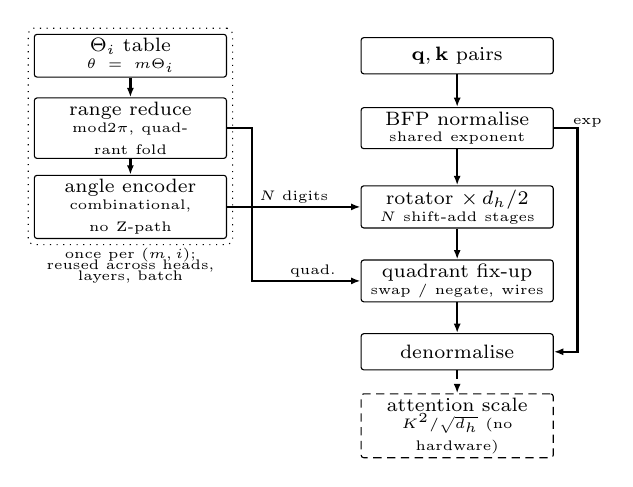
\begin{tikzpicture}[
  font=\scriptsize,
  box/.style   = {draw, rounded corners=1pt, align=center,
                  minimum height=4.6mm, inner xsep=2pt, inner ysep=1.5pt},
  wide/.style  = {box, text width=23mm},
  free/.style  = {box, densely dashed, text width=23mm},
  ar/.style    = {-{Latex[length=1.2mm]}, thick},
  lbl/.style   = {font=\tiny, inner sep=1pt}
]
\node[wide] (theta)  at (0,0)      {$\Theta_i$ table\\[-2pt]\tiny$\theta=m\Theta_i$};
\node[wide] (rr)     at (0,-0.92)  {range reduce\\[-2pt]\tiny$\bmod 2\pi$, quadrant fold};
\node[wide] (enc)    at (0,-1.92)  {angle encoder\\[-2pt]\tiny combinational, no Z-path};
\draw[ar] (theta) -- (rr);
\draw[ar] (rr)    -- (enc);
\begin{scope}[on background layer]
  \node[draw, dotted, rounded corners=2pt, inner sep=2pt,
        fit=(theta)(enc)] (fe) {};
\end{scope}
\node[lbl, anchor=north, align=center] at (fe.south)
      {once per $(m,i)$;\\[-2pt]reused across heads,\\[-2pt]layers, batch};
\node[wide] (qk)   at (4.15,0)      {$\mathbf{q},\mathbf{k}$ pairs};
\node[wide] (bfp)  at (4.15,-0.92)  {BFP normalise\\[-2pt]\tiny shared exponent};
\node[wide] (rot)  at (4.15,-1.92)  {rotator $\times\,d_h/2$\\[-2pt]\tiny $N$ shift-add stages};
\node[wide] (quad) at (4.15,-2.86)  {quadrant fix-up\\[-2pt]\tiny swap / negate, wires};
\node[wide] (den)  at (4.15,-3.76)  {denormalise};
\draw[ar] (qk)  -- (bfp);
\draw[ar] (bfp) -- (rot);
\draw[ar] (rot) -- (quad);
\draw[ar] (quad)-- (den);
\draw[ar] (enc.east) -- node[lbl,above]{$N$ digits} (rot.west);
\draw[ar] (rr.east)  -- ++(0.32,0) |- node[lbl,pos=0.78,above]{quad.} (quad.west);
\draw[ar] (bfp.east) -- ++(0.3,0)
          node[lbl,above right=-1pt and -3pt]{exp} |- (den.east);
\node[free] (gain) at (4.15,-4.70) {attention scale\\[-2pt]\tiny$K^{2}/\sqrt{d_h}$ (no hardware)};
\draw[ar,densely dashed] (den) -- (gain);
\end{tikzpicture}
\vspace{-4mm}
\caption{RoPE datapath. The angle front-end (dotted) depends on $(m,i)$ but
never on the data, so each digit string is reused across every head, layer and
batch element ($32\times32$ for a LLaMA-2-7B-class model). Digits are produced
combinationally, so no Z-path exists. Normalisation is functional, not
optional: measured activations reach $|q|=132$, $|k|=178$ against the $[-2,2)$
range of $Q(1,F)$. For Binary UD the scale factor never enters the datapath at
all; $K^{2}$ folds into the attention scale (dashed).}
\label{fig:arch}
\end{figure}

\subsection{The Angle Front-End}
\label{sec:encoder}

Fig.~\ref{fig:arch} shows the complete datapath. A UD stage rotates by
$a_i = \arctan(2^{-(i+1)})$, not by $2^{-(i+1)}$, so encoding a target angle is
a subset-sum over $\{a_i\}$ whose weights are only approximately geometric:
$a_i/2^{-(i+1)} = 0.927, 0.980, 0.995, 0.999,\ldots$ Reading digits straight
off the binary representation of $\theta$ (the construction the UD
formulation implies) therefore mis-encodes the leading stages, with an error
independent of pipeline depth. This is the defect, not the datapath: deepening
the pipeline does not fix it.

The tail is geometric to better than $0.13\%$, so it can be read from the
residual and only the two leading stages need explicit resolution. The encoder
is one adder, three constant comparators, a $4{:}1$ constant multiplexer and a
subtractor. It is fully combinational, so the Z-path-free property survives,
and at $N=10$ it reaches $0.094^{\circ}$ RMS against $2.20^{\circ}$ for the direct
construction, for $136$\,$\mu$m$^2$. Range reduction precedes it: $\theta$ is
reduced modulo $2\pi$ by truncation, which is exact and costs no adder, and the
quadrant is restored after the rotator by swaps and sign flips. The front-end
depends on $(m,i)$ but never on the data, so a digit string is computed once
and broadcast to every head, layer and batch element: $1024$ uses for a
LLaMA-2-7B-class model. It is \emph{not} shared across the $d_h/2$ pairs of a
head, since $\theta_i = m\Theta_i$ depends on $i$. This amortisation is what
makes a dedicated encoder affordable, and it is also why a bare multiplier
rotator is not a complete design: it consumes $\sin$ and $\cos$ that something
must still produce.

\subsection{Normalisation}
\label{sec:bfp}

A bare fixed-point rotator is not deployable. Query and key activations
captured from production models reach $|q| = 132$ and $|k| = 178$, against the
$[-2,2)$ range of $Q(1,F)$. Inputs are therefore block-normalised with a shared
exponent per (head, token) before the rotator and de-normalised after. This is
block floating point (BFP), chosen because the $d_h/2$ pairs of one head at one position
share a magnitude scale closely enough that one exponent serves them all.
Block size is a free parameter, and synthesis settles it against intuition:
covering one head's $64$ pairs costs $23877$\,$\mu$m$^2$ with a single shared
exponent against $22112$\,$\mu$m$^2$ as eight blocks of eight, which is also
$1.7\times$ more accurate and holds $293$\,ps of slack against $4$\,ps. We use
$D=8$; \S\ref{sec:precision} was measured at $D=64$ and is conservative for it.
Normalisation costs $345$\,$\mu$m$^2$ per pair at $W=14$, or $8\%$ of a
rotator, and applies equally to the multiplier and LUT baselines, so it does
not bias \S\ref{sec:hw}.

\subsection{Scale Factor and Its Compensation}
\label{sec:gain}

A shift-add micro-rotation is not a pure rotation: stage $i$ rotates by
$\arctan(2^{-(i+1)})$ and scales by $\sqrt{1+2^{-2(i+1)}}$, so over $N$ stages
\begin{equation}
  K = \textstyle\prod_{i=0}^{N-1}\sqrt{1 + 2^{-2(i+1)}},
  \label{eq:gain}
\end{equation}
which for $N=10$ is $K = 1.164435$. Conventional CORDIC removes this with a
compensation multiplier or extra scaling micro-rotations.

\subsubsection{RoPE does not pay for it}
Because $\delta_i \in \{-1,+1\}$ at every stage, \eqref{eq:gain} carries no
dependence on $\delta_i$ and $K$ is identical for every angle. Queries and keys
traverse the same rotator, so
\begin{equation}
  \frac{\langle K\mathbf{q}_m, K\mathbf{k}_n\rangle}{\sqrt{d_h}}
  = K^{2}\cdot\frac{\langle \mathbf{q}_m, \mathbf{k}_n\rangle}{\sqrt{d_h}},
  \label{eq:fold}
\end{equation}
and $K^{2}$, being independent of $m$, $n$ and the feature index, is absorbed
by replacing the attention scale $1/\sqrt{d_h}$ with $K^{2}/\sqrt{d_h}$. No
compensation hardware is required anywhere. RTL simulation gives a measured
output magnitude of $1.164426$ against $1.164435$ predicted, spread
$\pm 0.0003$ at $W=16$, confirming no angular dependence.

\subsubsection{Merging forfeits the property}
The argument fails for the merged datapath. A merged stage applies
$t = v\,2^{-2i}$ with $v$ drawn from a set containing more than one magnitude,
so its gain $\sqrt{1 + v^{2}4^{-i}}$ depends on the digit, hence on the angle;
for~\eqref{eq:merged} the accumulated gain ranges over $[1.00, 1.93]$. No
constant absorbs an angle-dependent factor, so~\eqref{eq:fold} does not apply.
This is not an artefact of the digit set: a digit-independent gain requires all
digits to share a magnitude, and a single-magnitude set carries one bit per
stage, which is Binary UD. \textbf{Constant gain and radix-4 stage merging
cannot be obtained together.}

\subsubsection{Recovering it cheaply}
The spread concentrates in the leading stages: stage $0$ accounts for
$80.3\%$ and stage $1$ for $6.8\%$. The head gain takes three distinct values,
so compensation reduces to selecting among three constants,
$K_{\text{head}}^{-1} \in \{1,\,0.707107,\,0.554700\}$, each a shift-add
network of three or four adders rather than a multiplier.

\begin{table}[t]
\caption{Gain compensation depth versus residual error and measured cost at
$W=14$. Perplexity is WikiText-2, full test split, $\mathrm{ctx}=2048$.}
\label{tab:gaincomp}
\centering
\begin{tabular}{lccccr}
\toprule
Compensated & Residual & \multicolumn{2}{c}{$\Delta$ perplexity} & Area & Merged \\
stages & spread & LLaMA-2 & Qwen2 & ($\mu$m$^2$) & total \\
\midrule
none      & $93.4\%$ & $+908.3\%$ & $+76.2\%$ & $0$    & 3467 \\
0 (H1)    & $7.3\%$  & $+0.62\%$  & $+0.77\%$ & 1032   & 4499 \\
0--1 (H2) & $0.47\%$ & $+0.005\%$ & $+0.008\%$& 1819   & 5286 \\
\bottomrule
\end{tabular}
\end{table}

Table~\ref{tab:gaincomp} settles the variant question. Full compensation brings
the merged datapath to $5286$\,$\mu$m$^2$, which is $940$\,$\mu$m$^2$
\emph{larger} than the $N$-stage Binary UD rotator that needs no compensation
and whose residual gain error is exactly zero, so H2 is strictly dominated. H1
survives only as an energy trade. Radix-4 merging therefore does not pay for
itself here: it saves $879$\,$\mu$m$^2$ of datapath at $W=14$, then forfeits
the property that makes the scale factor free and spends $1032$--$1819$\,
$\mu$m$^2$ buying a weaker version back.

\subsection{Synthesis Methodology}
\label{sec:method}

Operands use $Q(1,F)$: one sign bit, one integer bit and $F$ fractional bits,
so $W = F+2$. Both $F$ and $N$ are RTL parameters. Synthesis used Cadence Genus
21.10 targeting the \emph{Cadence GPDK045} 45\,nm library (\texttt{gsclib045})
with high- and low-$V_t$ cells alongside nominal $V_t$; physical libraries and
the QRC technology file were read, so areas are physical rather than wire-load
estimates. Every design ran the same flow under a 2.0\,ns constraint
(500\,MHz), combinational blocks against a matching maximum input-to-output
delay.

Two caveats bear on the absolute numbers. The corner is the library's
\emph{fast} corner, \texttt{fast\_vdd1v2} at PVT\_1P32V\_0C (1.32\,V,
0\,\textdegree C), which is optimistic relative to nominal. Every design,
including all baselines, used it, so the relative comparisons are unaffected.
Power comes from \texttt{report\_power} without switching-activity
back-annotation, which assumes uniform toggling and so understates the
shift-add advantage.

%% ===================================================================
\section{Results}
\label{sec:results}

\subsection{Precision Requirement}
\label{sec:precision}

Hardware behaviour is injected by replacing the rotary embedding with a
bit-accurate model of the synthesised datapath (the same encoder, range
reduction, block normalisation and pipeline), verified against RTL to
$0.002^{\circ}$. Only the \emph{rotation} is approximated; weights, activations
and the queries and keys stay in \texttt{float16}, so the numbers isolate the
rotation hardware rather than quantisation in general. Evaluation is the full
WikiText-2 raw test split, stride equal to context so each token is scored
once, KV cache disabled, batch 1, transformers 5.17.0 / torch 2.10.0.
Perplexity uses an explicit shift rather than passing \texttt{labels}, because
the framework applies its own and the two compose silently into an off-by-one
evaluation; absolute baselines should be read against the floating-point row of
the same table.

\begin{table}[t]
\caption{Perplexity versus fractional width $F$, Binary UD ($N=10$),
WikiText-2, $\mathrm{ctx}=2048$. $\Delta$ is relative to the
\texttt{float16} baseline of the same model.}
\label{tab:fsweep}
\centering
\begin{tabular}{ccccc}
\toprule
& \multicolumn{2}{c}{LLaMA-2-7B ($b{=}10^{4}$)} & \multicolumn{2}{c}{Qwen2-7B ($b{=}10^{6}$)} \\
\cmidrule(lr){2-3}\cmidrule(lr){4-5}
$F$ & PPL & $\Delta$ & PPL & $\Delta$ \\
\midrule
baseline & 5.4680 & ---        & 7.1405 & --- \\
11       & 5.4683 & $+0.005\%$ & 7.1417 & $+0.018\%$ \\
10       & 5.4691 & $+0.020\%$ & 7.1478 & $+0.103\%$ \\
9        & 5.4723 & $+0.078\%$ & 7.5943 & $+6.36\%$ \\
8        & 5.4854 & $+0.318\%$ & 16.527 & $+131\%$ \\
\bottomrule
\end{tabular}
\end{table}

The two models disagree, and the disagreement is the result.
Table~\ref{tab:fsweep} shows LLaMA-2-7B within $0.32\%$ of baseline at $F=8$,
degrading gracefully below. Qwen2-7B has already lost $6.4\%$ at $F=9$ and
collapses at $F=8$: two orders of magnitude across a single bit. A precision
adequate for one model is unusable for the other on identical hardware.

The cause is the frequency schedule, not model scale: both are 7B models with
the same head dimension. Qwen2 uses a RoPE base of $10^{6}$ against LLaMA-2's
$10^{4}$, so $\Theta_i = b^{-2i/d}$ spans a far wider dynamic range and the
low-frequency dimension pairs receive angles so small that the displacement
they produce falls below the datapath LSB. The limit is the data width, not
angular resolution: the angle datapath is held at $12$ fractional bits across
the whole sweep, and as $F$ falls the late rotator stages shift their operand
entirely below the LSB and cease to contribute. That pair then stops rotating
and its positional signal is discarded rather than degraded: a cliff rather
than a slope. Three further models at base $10^{4}$ track the LLaMA-2-7B column
within $0.05\%$ at every $F \ge 9$: the base, not the parameter count, is the
discriminator.

We therefore report no single optimum. \textbf{$F=11$ ($W=13$) is the
defensible recommendation for a general-purpose unit}, at $+0.005\%$ and
$+0.018\%$ on the two models, one bit above the point at which Qwen2 begins to
move; $F=10$ is the aggressive choice at $0.11\%$. A general-purpose
accelerator should provision for the wider base, since recent models trend
towards larger ones.

Rotation error does not accumulate with sequence length despite $\theta$
growing without bound: at $F=10$, degradation over contexts of $1024$, $2048$
and $4096$ is $+0.026/0.020/0.020\%$ for LLaMA-2-7B and
$+0.146/0.103/0.080\%$ for Qwen2-7B. Truncating modulo $2\pi$ is exact, so
error depends on the angle's position in the reduced range, not on $m$.

\subsection{Hardware Comparison}
\label{sec:hw}

\begin{table}[t]
\caption{Complete RoPE units synthesised on the same 45\,nm flow. Energy is
power at the 500\,MHz operating point. $\dagger$ marks a design that consumes
$\sin/\cos$ it does not generate, and is therefore not a complete unit.}
\label{tab:perf}
\centering
\resizebox{\columnwidth}{!}{%
\begin{tabular}{lrrrr}
\toprule
Design & Area & Power & Energy & Slack \\
       & ($\mu$m$^2$) & (mW) & (pJ/rot) & (ps) \\
\midrule
\multicolumn{5}{l}{\emph{$W=12$: the aggressive operating point}} \\
Std.\ CORDIC ($N{=}10$)      & 4669 & 4.208 & 8.42 & 1213 \\
Sin/cos LUT                  & 4047 & 3.308 & 6.62 & 201 \\
Multiplier$\dagger$          & 3092 & 1.540 & 3.08 & 648 \\
Binary UD ($N{=}10$)         & \textbf{3961} & 2.719 & 5.44 & \textbf{1499} \\
Merged UD ($N{=}5$) + H1     & 3828 & \textbf{1.551} & \textbf{3.10} & 1182 \\
\midrule
\multicolumn{5}{l}{\emph{$W=14$: FP16-matched datapath}} \\
Std.\ CORDIC ($N{=}10$)      & 5378 & 4.896 & 9.79 & 1174 \\
Sin/cos LUT                  & 5375 & 4.544 & 9.09 & 26 \\
Multiplier$\dagger$          & 4185 & 2.092 & 4.18 & 600 \\
Binary UD ($N{=}10$)         & \textbf{4346} & 2.805 & 5.61 & \textbf{1342} \\
Merged UD ($N{=}5$) + H1     & 4499 & \textbf{1.860} & \textbf{3.72} & 1105 \\
\bottomrule
\end{tabular}%
}
\end{table}

Table~\ref{tab:perf} reports every design synthesised under the identical flow,
library and constraint of \S\ref{sec:method}. The Binary UD rows reproduce the
earlier precision sweep exactly ($3961$ and $4346$\,$\mu$m$^2$), so all figures
here sit on one measurement basis.

\subsubsection{Against the standard CORDIC baseline}
At $W=14$ the Binary UD rotator is $19.2\%$ smaller and draws $42.7\%$ less
power than the standard CORDIC rotator of the same depth, with more timing
margin. The saving is the Z-path: an angle datapath, its registers and its
per-stage $\arctan$ table disappear, replaced by a digit pipeline and a shared
front-end costing $458$\,$\mu$m$^2$.

\subsubsection{What the multiplier row does and does not show}
The bare multiplier is the smallest entry at both word lengths, but it is not
a RoPE unit: it consumes $\sin$ and $\cos$ that something must still produce,
and the cost is visible in the table: the LUT row exceeds it by
$955$\,$\mu$m$^2$ at $W=12$ and $1190$\,$\mu$m$^2$ at $W=14$, precisely the
$\sin/\cos$ storage. \textbf{The LUT row is the completed multiplier design}.

Against it the two are comparable in area at $W=12$ ($3961$ against
$4047$\,$\mu$m$^2$, which we do not read as significant), but Binary UD
already uses $18\%$ less energy and holds $1499$\,ps of slack against
$201$\,ps. By $W=14$ the gaps open to $19.1\%$ in area and $38\%$ in energy,
the LUT holding $26$\,ps of margin against Binary UD's $1342$\,ps, and only
$30$\,ps at $W=16$: a shift-add pipeline grows as $\mathcal{O}(WN)$ while
table storage grows with both width
and angular resolution, so the advantage is in energy and timing at narrow
datapaths and becomes an area advantage only once the table does.

That the bare multiplier competes at all is explained by the register count,
not the arithmetic: twenty $W$-bit adders beat four $W\!\times\!W$
multipliers, but gate-level reports give the $W=14$ Binary UD rotator $363$
flip-flops, close to half its cell area, against a single-cycle
multiplier that pays almost none, so the $\mathcal{O}(W^2)$ term needs until
$W \approx 15$ to overcome that constant.

\subsubsection{Against prior RoPE hardware}
Neither published RoPE accelerator reports an absolute area or node, and each
measures against a different baseline, so we do not normalise them. Li
et al.~\cite{standard_cordic_rope} report $45.7\%$ area and $31.0\%$ power
saved against a fixed-point counterpart, agreeing in sign with our LUT
comparison rather than our bare-multiplier one, suggesting their baseline
includes $\sin/\cos$ generation. RoPIM~\cite{c23} reports $307.9\times$ speed
and $914.1\times$ energy against a GPU, on a substrate with no standard-cell
area. Every baseline in Table~\ref{tab:perf} is re-implemented here under one
flow, library and corner.

\subsubsection{Which variant}
Merged UD is the lowest-energy design at $3.72$\,pJ against $5.61$, and the
register accounting above is why: halving the pipeline halves the flip-flops.
It is not smaller once compensation is counted ($4499$ against
$4346$\,$\mu$m$^2$ at $W=14$) and carries a $0.6$--$0.8\%$ perplexity penalty
Binary UD does not, its gain error being zero by construction. We take Binary
UD as primary and merged UD as the variant for energy-dominated budgets.

\subsubsection{Throughput and integration}
Binary UD closes at $1.52$\,GHz at $W=14$; its $6.58$\,ns traversal is
immaterial because RoPE performs $128$ rotations per head, layer and token
against attention's $2N_{\text{ctx}}d_h$ multiply--accumulates, leaving one
rotator four times over-provisioned behind even a $512$-MAC datapath. The
rotations are $0.098\%$ of the attention arithmetic at $N_{\text{ctx}}=2048$,
and contribute no multipliers at all.

%% ===================================================================
\section{Conclusion}

We presented a multiplier-free, memory-free RoPE datapath on uniformly
distributed CORDIC, with three results specific to RoPE. The angle encoder the
UD formulation leaves unspecified is necessary and nearly free
($136$\,$\mu$m$^2$, $0.094^{\circ}$ RMS against $2.20^{\circ}$). The scale
factor is absorbed by attention at zero cost, but constant gain and radix-4
merging are mutually exclusive, and compensation costs more than merging
saves. Required precision follows the model's frequency schedule, not its
size. The rotator is $19.2\%$ smaller and $42.7\%$ lower in power than
standard CORDIC, and $19.1\%$ smaller with $38\%$ less energy than a
$\sin/\cos$ LUT. All RTL and scripts are released at~\cite{github}.

\balance
\bibliographystyle{IEEEtran}
\bibliography{references}

\end{document}
